%*******************************************************************************
%****************************** Second Chapter *********************************
%*******************************************************************************

\chapter{A new Peierls model}
\label{chap:peierls_model}
\graphicspath{{peierls_model/Figs/}}


Though there are a number \cite{Nabarro1947,Huntington1955, puls1976, Vitek1992,  Bulatov1997, Lubarda2007, Clegg2006,Gouriet2015} of Peierls models in the literature published over the decades since \citet{Peierls1940} first presented his short solution few have been adaptable to situations beyond the initially envisaged problem which is typically narrowly defined. In this chapter a model is presented that allows, with a minimum of effort, the consideration of energies defined by linear elasticity, empirical potentials, generalised stacking fault energies and which could be extended to a full quantum mechanical treatment, using density functional theory.

The python programming language was chosen for a number of reasons, firstly the python model is inherently modular, which provides a flexible structure, allowing parts of the model to be altered, extended or replaced quickly easily. Python is also widely used with a large body of documentation and a large support community. Finally python has a very large number of extending modules providing advanced capabilities, particularly projects like NumPy and SciPy. NumPy provides a powerful and efficient implementation of arrays providing a range of simple functions as well as more advanced linear algebra operations. SciPy is a project built on the basic data structure of the numpy array and provides advanced algorithms and convenience functions including differential equations, numerical solvers and optimisers, image processing and statistical functions.


To calculate the Peierls stress we must find the energy of dislocation configurations as the dislocation is displaced from one equilibrium position to the next. The variable $\alpha$ is used to denote the fractional displacement of the dislocation. Since boundary conditions are insufficient to define the atomic configuration, for each value of $\alpha$ the atomic configuration of the dislocation that minimises the energy must be found. Once a sufficient samples of $\alpha$ have been made the Peierls stress can be calculated by 

\begin{equation}
\tau_p = \frac{1}{lb^2}   \left. \frac{\partial U}{\partial \alpha} \right|_{max} .
\end{equation}

Where $l$ is the length of dislocation line for which the energy, $U$, is calculated for and $b$ is the Burgers vector.

So for a given value of alpha how can the ideal, that is lowest energy, configuration be found? This requires two steps, first the definition, creation and representation (as a data structure) of a configuration and second the evaluation of the energy thereof.
Taken together these can be thought of as a simple function that takes the value of $\alpha$ along with some input parameters as arguments and returns the energy:

\begin{equation}
U = f(\alpha, p_1, p_2,...,p_n )
\label{eqn:energy_as_function}
\end{equation}

The input parameters, $p_i$, could be as general as the coordinates of every atom in the configuration or as specific as the single parameter defined by by Peierls in his original treatment, the width of the dislocation, the only difference is one of computational tractability. Algorithms exist for finding the minimum of functions of the form given in \autoref{eqn:energy_as_function} but they are much faster for functions with small numbers of parameters and some algorithms are not reliable for large numbers of parameters, hence decisions about how to define an atomic configuration will have consequences for the optimisation of that configuration.

A sensible approach is to use the most general representation of a dislocation and then apply constraints to it rather than find the model limited by an assumption of specificity later. Hence individual atoms are represented in space by coordinates as an array of the form:

$$ atoms = \begin{pmatrix}
x_1 & y_1 & z_1  \\
x_2 & y_2 & z_2  \\
.   &.    &.     \\
.   &.    &.     \\
x_n & y_n & z_n  \\
\end{pmatrix}
$$

Where $x$, $y$ and $z$ are coordinates in euclidean space in units of \r{A}ngstr\"{o}ms, i.e. \emph{not} relative to any crystallographic axes.

This representation can be extended, for example in the case of ionic solids the charge on each ion would be a necessary parameter for any energy calculation, this would be represented thus:
$$
atoms = \begin{pmatrix}
x_1 & y_1 & z_1 & q_1 \\
x_2 & y_2 & z_2 & q_2 \\
.   &.    &.    &.    \\
.   &.    &.    &.    \\
x_n & y_n & z_n & q_n \\
\end{pmatrix}
$$
This could be extended to an arbitrary number of parameters such as parameters for empirical potentials, labels for symmetrical distinct ions of the same species etc.





\section{Building a dislocation}
\FloatBarrier
\label{sec:build}




The model might be expected to start in the same way as Peierls; bringing together two half crystals as shown in \autoref{fig:semi_infinite_crystals} and simply allowing the structure to relax, leaving all the atomic positions as free variables. However there are two reasons to apply constraints to the atomic coordinates. Firstly constraints reduce the number of parameters to search. Secondly an unconstrained global optimiser might remove the dislocation entirely to create a perfect crystal, since dislocations are not equilibrium defects the most stable configurations for the atoms would be in a defect free crystal. To achieve this a displacement field based on initial atomic coordinates is used to find a final atomic configuration.

For a given value of $\alpha$ there will be an initial configuration of atoms defined by two half crystals brought together at a slip plane with some relative displacement between them defined by $\alpha$ and the Burgers vector. The core of the dislocation is taken to be the line where $x,y = 0$. The position of the core with respect to the lattice of the half crystals is defined by $\alpha$, usually with $\alpha=0$ defining the configuration in which the extra half-plane of atoms aligns with the dislocation core, as shown in \autoref{fig:joined_half_crystals}. 

The final, in the sense of ready to be evaluated energetically rather than optimised, configuration is the combination of  the initial positions and an array of displacements defined by some displacement field, $\bm{\delta}(x_0, y_0, z_0)$, i.e.
\begin{equation}
\mathbf{r}_i = \mathbf{r}_i^0 + \bm{\delta}(\bm{r}_i^0)
\end{equation}
where $\mathbf{r}_i$ is the position vector defining the final position of the $i$th atom, $\mathbf{r}_i^0$ is the vector defining the initial position of the $i$th ion and $\bm{\delta}$ is a vector displacement field.


%%%%%%%%%%%%%%%%%%%%%%%%%%%%%%%%%%%%%%%%%%%%%%%%%%%%%%%%%%%%%%%%%%%%%%%%%%%5
%
%                      Initial half crystals
%
%%%%%%%%%%%%%%%%%%%%%%%%%%%%%%%%%%%%%%%%%%%%%%%%%%%%%%%%%%%%%%%%%%%%%%%%%%%%%%
\subsection{Defining the initial atomic positions}


Firstly we must define the initial positions of the atoms in the half crystals. In the Peierls model the material was assumed to be a simple orthorhombic lattice; i.e. a misaligned  bond across the slip plane has a minimum energy when the bond is normal to the slip plane. To consider the effects of the particular structure the atomic configuration must be generated from the lattice and motif of the perfect crystal.

To create a crystal conveniently oriented with respect to the Cartesian reference axes and the crystal slip system unconventional unit cells were defined. Directions and planes defined relative to the unconventional or dislocation cell will be marked prime, e.g. $[1\,0\,0]'$. The Burgers vector $\mathbf{b}$ is taken to be the $[1\,0\,0]'$, the shortest slip plane normal that is a full lattice vector is taken to be $[0\,1\,0]'$ and the $[0\,0\,1]'$, parallel to the line vector, is the shortest lattice vector that is perpendicular to both the Burgers vector and the slip plane normal and its sign is such that the axes are right handed. Filling space by combining a motif and a lattice defined according to these axes is convenient because most of the mathematical results of dislocation theory, stress and strains fields etc., are defined taking $x$, $y$ and $z$ parallel to $[1\,0\,0]'$, $[0\,1\,0]'$, $[0\,0\,1]'$ respectively.

For example the \ce{NaCl} <1\,\={1}\,0>\{1\,1\,0\} slip system gives a new unit cell aligned with the slip system:

\begin{equation*}
\begin{aligned}[c]
{[1\,0\,0]}' &=\, ^{1}\!/_{2} [1\,1\,0]   \\
{[0\,1\,0]}' &=\, ^{1}\!/_{2} [1\,\overline{1}\,0]   \\
{[0\,0\,1]}' &=\, [0\,0\,1]   
\end{aligned}[c]
\qquad
\begin{aligned}[c]
&\parallel \mathbf{b} \\
&\parallel \mathbf{d} \\
&\parallel \mathbf{l}
\end{aligned}
\end{equation*}
where $\mathbf{l}$ is the line vector of the dislocation.


The atoms in this non-conventional unit cell are
$$
motif = \begin{pmatrix}
0 & 0 & 0 & +1 \\
^{1}\!/_{2} & ^{1}\!/_{2} & ^{1}\!/_{2} & +1 \\
0 & 0 & ^{1}\!/_{2} & -1 \\
^{1}\!/_{2} & ^{1}\!/_{2} & 0 & -1 \\
\end{pmatrix}
$$
where a $+1$ in the final column denotes the positive charge of a sodium ion and a $-1$ denotes the negative charge of a chloride ion.



\begin{figure}
\centering


    \begin{subfigure}{0.55\textwidth}
    \centering
    \includegraphics[width=\textwidth]{NaCl_conventional_unit_cell}
    \caption{The conventional unit cell of sodium chloride with the salient slip directions and plane normals highlighted. \label{fig:NaCl_conventional_cell_slip_system_marked}}
    \end{subfigure}

    \begin{subfigure}{0.4\textwidth}
    \centering
    \includegraphics[height=2.0in]{NaCl_110_110}
    \caption{The sodium chloride unit cell best aligned with the <1\,1\,0>\{1\,\={1}\,0\} slip system. \label{fig:NaCl_110_110_unit_cell}}
    \end{subfigure}
    ~
    \begin{subfigure}{0.4\textwidth}
    \centering
    \includegraphics[height=2.5in]{NaCl_110_001}
    \caption{The sodium chloride unit cell best aligned with the <1\,1\,0>\{0\,0\,1\} slip system. \label{fig:NaCl_110_001_unit_cell}}
    \end{subfigure}

\caption[Unconventional unit cells of rock salt to build a dislocation.]{Possible unit cells for sodium chloride showing the conventional unit cell and two unconventional unit cells with the new crystallographic axes aligned to slip system, i.e. the Burgers vector and slip plane normal.\label{fig:unconventional_NaCl_unit_cells}}
\end{figure}






Similarly the \ce{NaCl} <1\,\={1}\,0>\{0\,0\,1\} slip system is defined by the unit cell:
\begin{equation*}
\begin{aligned}[c]
 {[1\,0\,0]}' &=\, ^{1}\!/_{2} [1\,1\,0] \\
 {[0\,1\,0]}' &=\,  [0\,0\,1] \\
 {[0\,0\,1]}' &=\; ^{1}\!/_{2} [1\,\overline{1}\,0] \\
\end{aligned}
\qquad
\begin{aligned}[c]
&\parallel \mathbf{b} \\
&\parallel \mathbf{d} \\
&\parallel \mathbf{l}
\end{aligned}
\end{equation*}
and the atoms are
$$
motif = \begin{pmatrix}
0 & 0 & 0 & +1 \\
^{1}\!/_{2} & ^{1}\!/_{2} & ^{1}\!/_{2} & +1 \\
^{1}\!/_{2} & 0 & ^{1}\!/_{2} & -1 \\
0 & ^{1}\!/_{2} & 0 & -1
\end{pmatrix}
$$


These unit cells are shown in relation to the conventional cell in \autoref{fig:unconventional_NaCl_unit_cells}. With these unit cells we can convolve the motif with a lattice to generate an initially perfect crystal defined with respect to Cartesian axes aligned with the slip system. Two offsets are then applied; firstly the half crystal below the slip plane, which is defined by $y < 0$, will be offset in the positive $x$ direction by $b/2$ and then the entire crystal is offset to put the dislocation core in the desired location. The latter will require an offset along the slip direction, $[0\,0\,1]'$ of $\alpha b$ and an additional offset in the $[0\,1\,0]'$ direction. While the magnitude of this offset is not necessarily predictable in the case of \ce{NaCl} the core must be at a height of $d/4$ in order to be halfway between the two (0\,2\,0) layers.

So the initial positions of the atoms in the dislocated crystal are related to those of an initially perfect crystal by
\begin{equation}
\bm{r_i^0} = \bm{r_i^{\text{perfect}}} +\begin{cases}
[-\alpha{}b, h, 0] & \quad \text{if } y_i^{\text{perfect}} > 0\\
[b(1/2 - \alpha{}), h, 0] & \quad \text{if } y_i^{\text{perfect}} < 0\\
\end{cases} 
\end{equation}

The offset to the atomic coordinates in $-\alpha{}b$ such that as $\alpha$ increases the dislocation motion is in the positive $x$ direction.





\FloatBarrier












%%%%%%%%%%%%%%%%%%%%%%%%%%%%%%%%%%%%%%%%%%%%%%%%%%%%%%%%%%%%%%%%%%%%%%%%%%%%%%%%%%%

                          % Displacement fields

\subsection{Displacement fields}

A suitable displacement field is required. First we can take a Volterra dislocation, which in a continuous isotropic elastic medium has a displacement field \cite{hirth_lothe1982volterra_displacements}:
\begin{subequations}
\begin{align}
u^x &= \frac{b}{2\pi}\left[ \arctan\left(\frac{x}{y}\right) + \frac{xy}{2(1-\nu)(x^2 + y^2)} \right] \\[0.5ex]
v^y &= -\frac{b}{2\pi} \left[ \frac{1-2\nu}{4(1-\nu)} \ln(x^2 + y^2) + \frac{x^2 + y^2}{4(1-\nu)(x^2 + y^2)} \right]
\end{align}
\end{subequations}
where $u^x$ and $v^y$ are the components of the displacement field parallel to $x$ and $y$ respectively, $x$ is the initial position parallel to the Burgers vector, $y$ is the initial position parallel to the slip plane normal, $b$ is the magnitude of the Burgers vector and $\nu$ is the Poisson ratio of the material. The terms all converge to fixed values at large $x$ or $y$ except the logarithmic component of $v^y$. This represents the bending of a single crystal that arises from the introduction of an extra half plane \cite{hirth_lothe1982volterra_displacements}.

This formulation of the displacement field and subsequent solution for an isotropic elastic continuum is discontinuous, diverging at $r=0$, where $r=\sqrt[]{x^2+y^2}$. To remove the discontinuity \citet{Eshelby1949} proposed considering a single dislocation to be composed of a continuous distribution of dislocations with infinitesimal Burgers vectors, the integral of which yields the Burgers vector of the full dislocation. 

By considering the local strains (a normal strain parallel to the slip plane) due to this distribution and integrating the stress on the slip plane can be found. By applying a force balance condition with the misalignment term the displacements at the slip plane can be found:


If $\bm{b}'(x')\mathrm{d}x'$ is the Burgers vector of an infinitesimal dislocation between $x'$ and $x'+\mathrm{d} x'$, and displacements in $y$ are assumed to be small, this can be related to the displacement, $u^x$, since the local displacement will be given by $-2(\mathrm{d} u^x/\mathrm{d} x)\mathrm{d} x'$ \cite{hirth_lothe1982peierls_displacements} we can write


\begin{equation}
b = \int_{-\infty}^{\infty} b'(x') \dd x' = -2\int^{\infty}_{-\infty} \left( \! \frac{\dd u^x}{\dd x} \right)_{x=x'} \dd x' 
\end{equation}
Using the result for a Volterra dislocation \cite{hirth_lothe_1982_volterra_stress_field}:
\begin{equation}
\sigma^{\text{Volterra}}_{xy} = \frac{\mu b}{2\pi (1-\nu)} \frac{x(x^2 - y^2)}{(x^2+y^2)^2}
\end{equation}
and setting $y=0$,
\begin{equation}
\sigma^{\text{volterra}}_{xy}(x,0) = -\frac{\mu}{2\pi(1-\nu)} \int^{\infty}_{-\infty} \frac{b'}{x-x'} \!\dd x' =  \frac{\mu}{\pi(1-\nu)} \int^{\infty}_{-\infty} \frac{1}{x-x'} \left(\!\frac{\dd u^x}{\dd x}\right)_{x=x'} \!\dd x'
\label{eqn:elastic_stress_at_slip_plane}
\end{equation}

At the minimum energy position the net stress at $(x,0)$ vanishes, so there must be a balancing stress arising from the misalignment of the material across the slip plane. By analogy with \citet{Frenkel1926}
\begin{equation}
\sigma_{xy}^{\text{misalignment}}(x,0) = C \sin \left( \frac{2\pi \phi^x}{b} \right)
\end{equation}
or in terms of the displacements either side of the slip plane:
\begin{equation}
\sigma_{xy}^{\text{misalignment}}(x,0) = -C \sin \left( \frac{4\pi u^x}{b} \right)
\end{equation}
If Hooke's law is satisfied at small strains we can write
\begin{equation}
\sigma_{xy}^{\text{misalignment}}(x,0) = 2 \mu \varepsilon_{xy} = \frac{\mu{}\phi^x}{d}
\label{eqn:misalign_stress_at_slip_plane}
\end{equation}
We can combine \autoref{eqn:elastic_stress_at_slip_plane} and \autoref{eqn:misalign_stress_at_slip_plane} to give a integral equation thus:
\begin{equation}
\int^{\infty}_{-\infty} \frac{1}{x-x'} \left(\!\frac{\dd u^x}{\dd x}\right)_{x=x'} \dd x' = \frac{b(1-\nu)}{2d} \sin\left(\frac{4\pi{}u^x}{b}\right)
\end{equation}
The solution is \cite{hirth_lothe1982peierls_displacements,Eshelby1949}
\begin{equation}
u^x(x) = -\frac{b}{2\pi} \arctan \left( \frac{x}{w} \right)
\label{eqn:one_dimensional_displacements}
\end{equation}
where $w$ is the half width of the dislocation and, for an isotropic elastic solid, has the value
\begin{equation}
w = \frac{d}{2(1-\nu)}.\label{eqn:half_width}
\end{equation}
\autoref{eqn:one_dimensional_displacements} satisfies the boundary condition that $u^x(\infty) = - u^x(-\infty) = -b/4$. Also $x=w$ gives $u^x(w)=1/2\, u^x(\infty)$, i.e. in the region $-w < x < w$ the disregistry across the slip plane is greater than half the maximum that occurs at $x=0$.

The two dimensional case gives a displacement field \cite{Eshelby1949,Leibfried1949,nabarro1987theory}:
\begin{subequations}\label{eqn:displacements}
\begin{align}
u^x(x,y) &= \frac{b}{2\pi} \left( \arctan \left[ \frac{y +  w\frac{|y|}{y}}{x} \right] - \frac{\pi}{2} \frac{|y|}{y} \frac{|x|}{x} \right) + c_1 \frac{xy}{x^{2} + (y + w\frac{|y|}{y} )^2} \\
v^y(x,y) &= c_2 \frac{y(y +  w \frac{|y|}{y})}{x^2 + (y +  w \frac{|y|}{y})^2} + c_3 \ln \left| \frac{x^2 + (y +  w \frac{|y|}{y})^2}{b^2} \right|
\end{align}
\label{eqn:displacement_field}
\end{subequations}
The final atomic configuration is then defined by 
\begin{equation}
\bm{r}_i = \bm{r}_i^0 + [u_i^x\,\bm{\mathrm{\hat{i}}},\; v_i^y\,\bm{\mathrm{\hat{j}}},\; 0\,\bm{\mathrm{\hat{k}}}]
\end{equation}

These terms can be interpeted physically; The arctan term is the same as in the original Peierls treatment, representing displacements along the slip plane that alter the local misalignment acorss the slip plane. The terms with the prefactors $c_1$ and $c_2$ represent shear strains, the $xy$ and $yx$ shears respectively. The logarithmic term, with the prefactor $c_3$, represents the bending of the entire crystal that must arise from the introduction of an extra halfplane of atoms. This logarithmic term does not converge to a constant value at large $x$ or $y$, but this is consistent with this physical interpretation \cite{hirth_lothe1982peierls_displacements}.

The inclusion of $v^y(x,y)$ in the displacement field means that there will always be some finite displacement normal to the slip plane. This is expected and will be associated with phenomena such as pressure dependent yield stress \cite{frost1982pressure}. These displacements might also be responsible for the normal strains observed around line defects in layered crystals that have been ascribed to ripplocations \cite{Gruber2016}.




For an isotropic elastic medium the various parameters in \ref{eqn:displacement_field} are analytically found to have fixed values for the lowest energy dislocation. The half-width, $w$, takes the same value as in \autoref{eqn:half_width} and the three other parameters are defined by
\begin{subequations}\label{eqn:disloc_params}
\begin{align}
c_1 &= \frac{b}{4\pi{}(1-\nu)} \\
c_2 &= \frac{b}{4\pi{}(1-\nu)} \\
c_3 &= - \frac{b(1-2\nu)}{8\pi(1-\nu)}.
\end{align}
\label{eqn:expressions_for_the_ideal_disloca_parameters}
\end{subequations}
The terms of the form $|x|/x$ and $|y|/y$ are to give all the terms the right sense in the right regions of space, i.e. above and below the slip plane in $y$ and either side of the dislocation in $x$. This reduces to the simpler solution in \autoref{eqn:one_dimensional_displacements} if only the atoms adjacent to the slip plane are considered. This form is useful because it is continuous and finite for all values of $x$ and $y$. 


\begin{figure}
\centering

    \begin{subfigure}{0.4\textwidth}
    \centering
    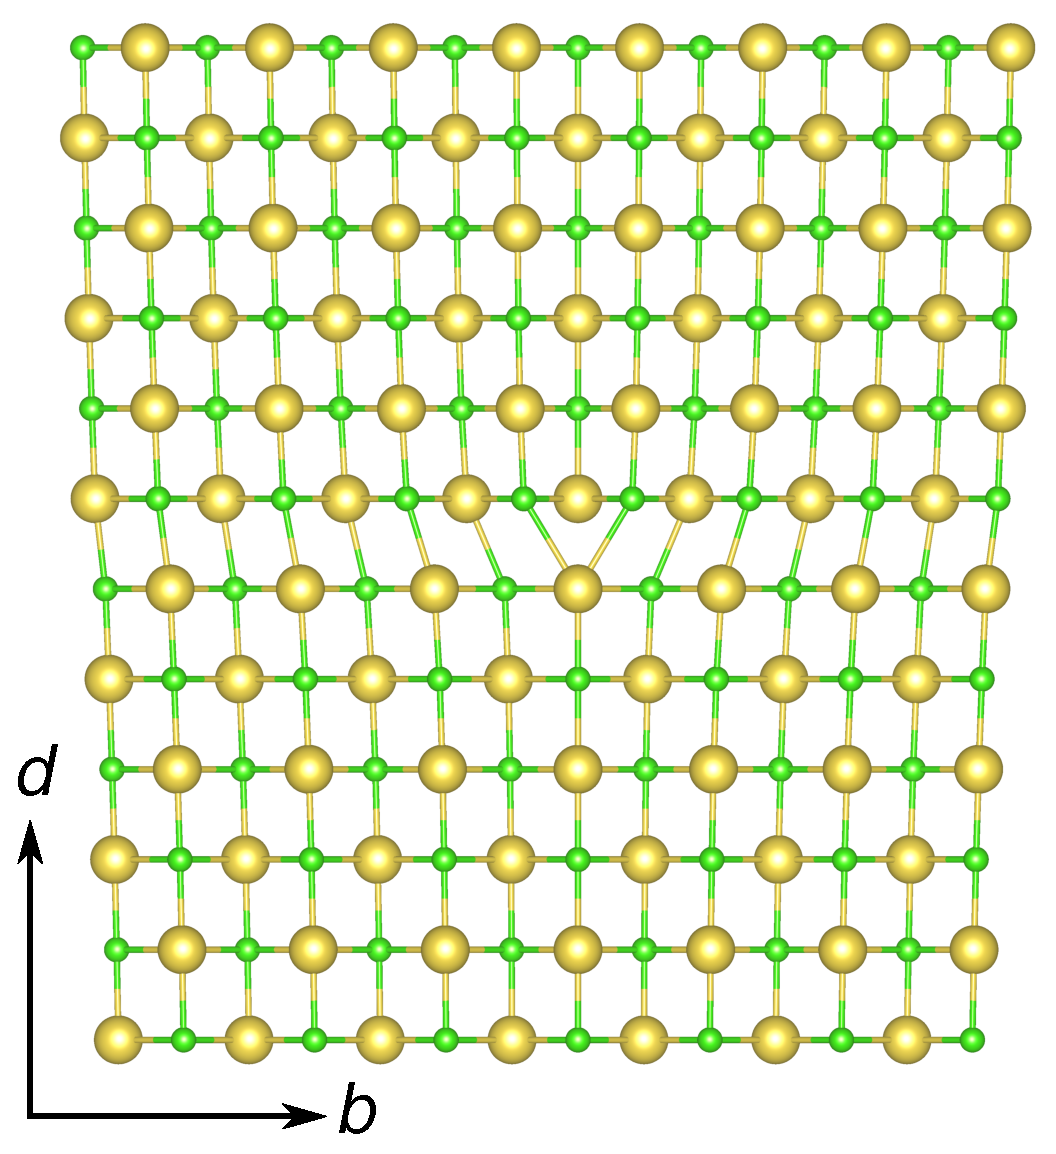
\includegraphics[width=0.6\textwidth]{wide_NaCl}
    \caption{A dislocation with a large width.}
    \end{subfigure}
    ~
    \begin{subfigure}{0.4\textwidth}
    \centering
    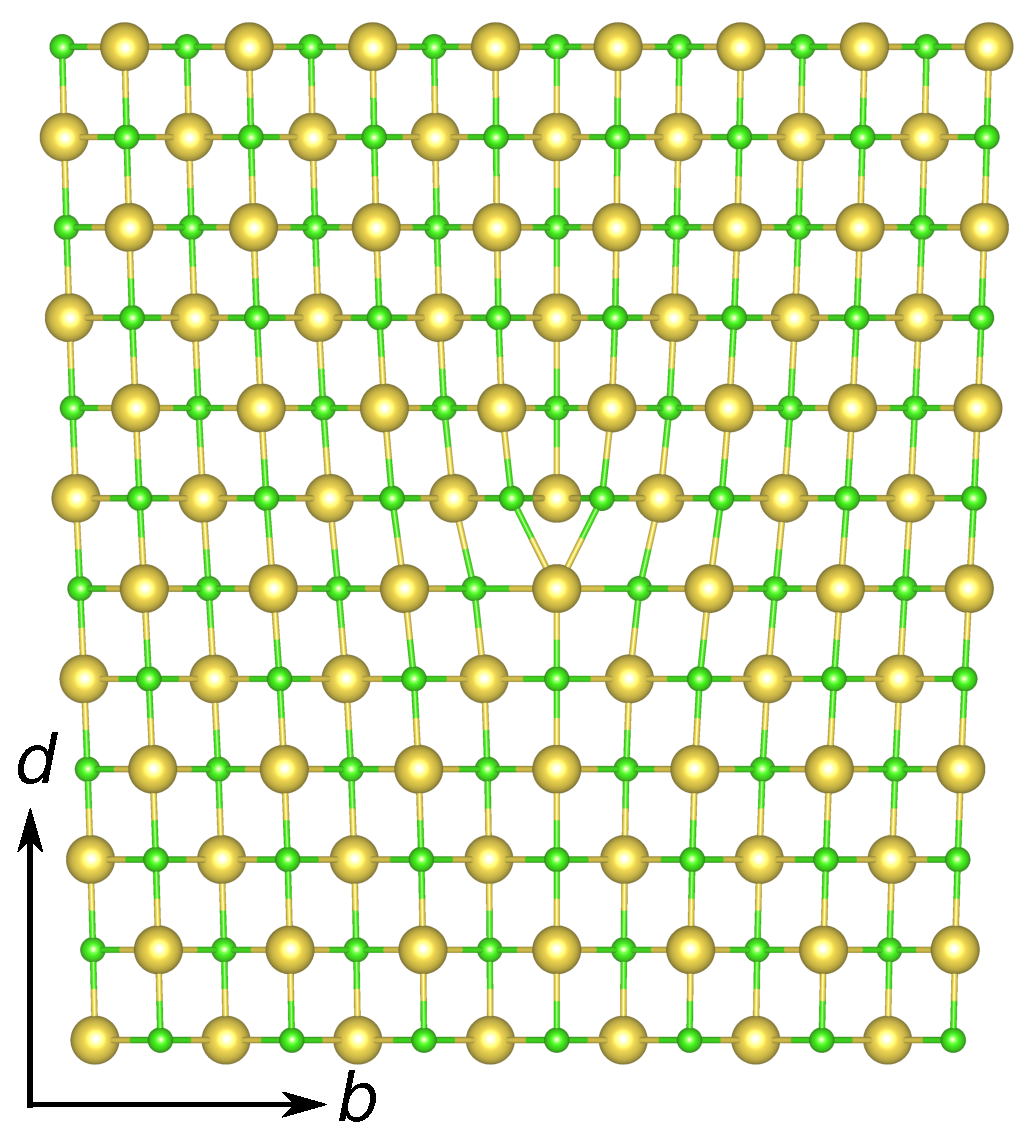
\includegraphics[width=0.6\textwidth]{narrow_NaCl}
    \caption{A dislocation with a small width.}
    \end{subfigure}

	\begin{subfigure}{0.4\textwidth}
	\centering
    \includegraphics[width=0.6\textwidth]{large_c1_NaCl}
    \caption{Large values of $c_1$ and $c_2$.}
	\end{subfigure}
    ~
	\begin{subfigure}{0.4\textwidth}
	\centering
    \includegraphics[width=0.6\textwidth]{large_c3_NaCl}
    \caption{A large value of $c_3$.}
	\end{subfigure}

    \begin{subfigure}{0.8\textwidth}
    \centering
    \includegraphics[width=0.5\textwidth]{typical_NaCl}
    \caption{A ``typical'' configuration.}
    \end{subfigure}

\captionsetup{width=0.8\textwidth}
\caption[The displacement field around an edge dislocation in rock salt.]{Various configurations of sodium chloride <1\,1\,0>\{0\,0\,1\} dislocations demonstrating the effects of the parameters of the displacement field defined in \autoref{eqn:displacements}, $w$, $c_1$, $c_2$ and $c_3$. Typical parameters are taken to be those predicted for an isotropic elastic material as given in  Equations~\ref{eqn:half_width} and \ref{eqn:disloc_params}, giving \SI{1.78}{\angstrom}, \SI{0.40}{\angstrom}, \SI{0.40}{\angstrom} and \SI{-0.12}{\angstrom} respectively for sodium chloride. Exaggerated values were ten times that. Calculated with $\nu =$~\num{0.207} and $a =$~\SI{5.644}{\angstrom} \cite{Theocaris1994,Rao1990}.\label{fig:parameters_of_the_disloc_configuration}}
\end{figure}


This gives a displacement field for a general material in which has four parameters; the width, $w$, and the scaling factors, $c_1$, $c_2$ and $c_3$. These parameters are varied to find the lowest energy dislocation. If the energy is calculated by an atomistic model, rather than by continuum elasticity, then there is no analytical solution for these parameters. Instead those values that minimise the energy are taken to be the correct solution.

The width of the dislocation still defines the region with large disregistries, while $c_1$ and $c_2$ define the magnitude of displacements associated with shear strains around the dislocation core and $c_3$ defines the magnitude of the bending of a crystal that must arise from the introduction of an extra half plane.
To illustrate the displacements produced by these different terms some exaggerated dislocation configurations are shown in \autoref{fig:parameters_of_the_disloc_configuration}.





A final note on the parametrisation of the dislocation structure is that the values $c_1$, $c_2$ and $c_3$ are not constrained. The purely isotropic case described above the parameters $c_1$, $c_2$ are positive and $c_3$ is negative, but there is no physical reason they cannot have a different sign. However a negative value of the width is not meaningful in this formulation. A negative width reintroduces the discontinuity at which displacements would diverge (in fact it would introduce two, one either side of the slip plane) which cannot be actually exist. Hence the constraint that $w>0$ is applied, but $c_1$, $c_2$ and $c_3$ are allowed to vary freely.





































\section{Evaluating the dislocation energy}
\label{sec:dislocation_energy}



Since there are insufficient boundary conditions to completely define a dislocation configuration with even four parameters the energy of the dislocation is the only way to identify a``correct'' or true configuration. Hence we must characterise the energy of arbitrary configurations. One obvious method to calculate the energy is to try and replicate the model based on elastic energy in the two half crystals and misalignment energy across the slip plane, there is the opportunity to calculate the full strain tensor and along with single crystal elastic constants the effects of elastic anisotropy can be taken into account. Another would be to use empirical potentials similar to those used in molecular dynamics; this would allow the exploration of dislocation properties in materials that are not well modelled by elasticity, ionic solids or compound semiconductors are examples of materials where elasticity is probably less appropriate. Both of these approaches are explored.

\subsection{Strain energy and misalignment energy}

This approach builds on the original approach of \citet{Peierls1940} and then \citet{Nabarro1947} and explains how the dislocation is stable due to a balancing of two forces, there is a force that attempts to spread the dislocation out into a planar defect, this arises due to the elastic stored energy in the bonds either side of the slip plane which would be zero in the case of a planar defect, which can be described by an infinitely wide dislocation. The other force tends to narrow the dislocation, this arises due to the misfit or misalignment across the slip plane. This would be a maximum for the planar defect where the entire slip plane is misaligned and would decrease monotonically as the width decreases.

Using this approach to the energy has a number of advantages. A two dimensional model is sufficient since for a long dislocation the condition of plane strain can be applied. If elastic theory can be applied at the scale of the unit cell then displacements need only be considered between unit cells rather than within them, which simplifies the model considerably.

\subsubsection{Strain energy}

Firstly the elastic energy can be easily calculated for a small volume if the strain and the elastic tensor is known. A good discussion of tensors and elasticity is given by \citet{kelly_knowles2012chapter5_tensors,kelly_knowles2012chapter6_stress_strain} and a discussion of elasticity in the context of dislocation theory is given by \citet{hirth_lothe1982elasticity}. The salient results are drawn together here.

Hookes law can be written as a tensor relationship using the einstein summation convention:
\begin{equation}
\sigma_{ij} = c_{ijkl} \epsilon_{kl}
\end{equation}
where $\sigma_{ij}$ is the stress tensor, $c_{ijkl}$ is the elastic tensor defining the properties of the material and $\epsilon_{kl}$ is the strain tensor. Strain is defined, for $i=j$, by
\begin{equation}
\epsilon_{ii} = \frac{\partial u_i}{\partial x_i}
\end{equation}
and for $i\neq j$ by
\begin{equation}
\epsilon_{ij} = \frac{1}{2} \left( \frac{\partial u_i}{\partial x_j} + \frac{\partial u_j}{\partial x_i} \right).
\end{equation}
%In Voigt notation the equation can be written
%\begin{equation}
%\sigma_i = c_{ij} \epsilon_{j}
%\end{equation}
%where 
%\begin{equation}
%\sigma_i = \begin{bmatrix}
%\sigma_{11} \\
%\sigma_{22} \\
%\sigma_{33} \\
%\sigma_{23} \\
%\sigma_{31} \\
%\sigma_{12} 
%\end{bmatrix}
%\qquad\qquad
%\epsilon_i = \begin{bmatrix}
%\epsilon_{11} \\
%\epsilon_{22} \\
%\epsilon_{33} \\
%\gamma_{23} \\
%\gamma_{31} \\
%\gamma_{12} 
%\end{bmatrix}
%\end{equation}
%This allows the reduction of the $3\times3\times3\times3$ tensor $c_{ijkl}$ to a $6\times6$ matrix $c_{ij}$. Note that to preserve the symmetry across the leading diagonal in $c_{ij}$ the strain components for $i\neq j$ are defined by $\gamma_{ij} = 2 \epsilon_{ij}$.
If Hooke's law holds then the stored elastic energy per unit volume is
\begin{equation}
u_{\text{elastic}} =\, ^{1}\!/_{2}\, \sigma_{ij} \epsilon_{ij} =\, ^{1}\!/_{2}\, c_{ijkl} \epsilon_{ij} \epsilon_{kl}.
\end{equation}
Hence to find the elastic energy we must evaluate \({\partial u_i}/{\partial x_j}\) for $i, j = 1, 2, 3$.
Assuming that we consider displacements between unit cells, and not within them, and assuming an orthogonal lattice estimating the components of strain is not difficult. The  condition of plane strain constrains $\epsilon_{ij} = 0$ for $i\, \text{or}\, j=3$. In the $1$--$2$ (or $x$--$y$) plane the strains can be identified from the vectors between neighbouring unit cells. For simplicity a primitive lattice is assumed and these vectors can be conceived of as bonds.

For this simple case for each atom two bonds are identified, one to the nearest neighbour in the $x$~direction and one to the nearest neighbour in the $y$~direction as shown in \autoref{fig:bonds}. The simplest estimate of the stress components is
\begin{alignat}{2}\label{eqn:estimate_strains}
\left. \frac{\partial u_x}{\partial x}\right|_i &= \frac{\mathbf{p}_i \cdot \mathbf{\hat{i}}}{b} &\qquad\qquad
\left. \frac{\partial u_x}{\partial y}\right|_i &= \frac{\mathbf{q}_i \cdot \mathbf{\hat{i}}}{d} \nonumber\\
\left. \frac{\partial u_y}{\partial y}\right|_i &= \frac{\mathbf{q}_i \cdot \mathbf{\hat{j}}}{d} &
\left. \frac{\partial u_y}{\partial x}\right|_i &= \frac{\mathbf{p}_i \cdot \mathbf{\hat{j}}}{b}
\end{alignat}


\begin{figure}
\centering
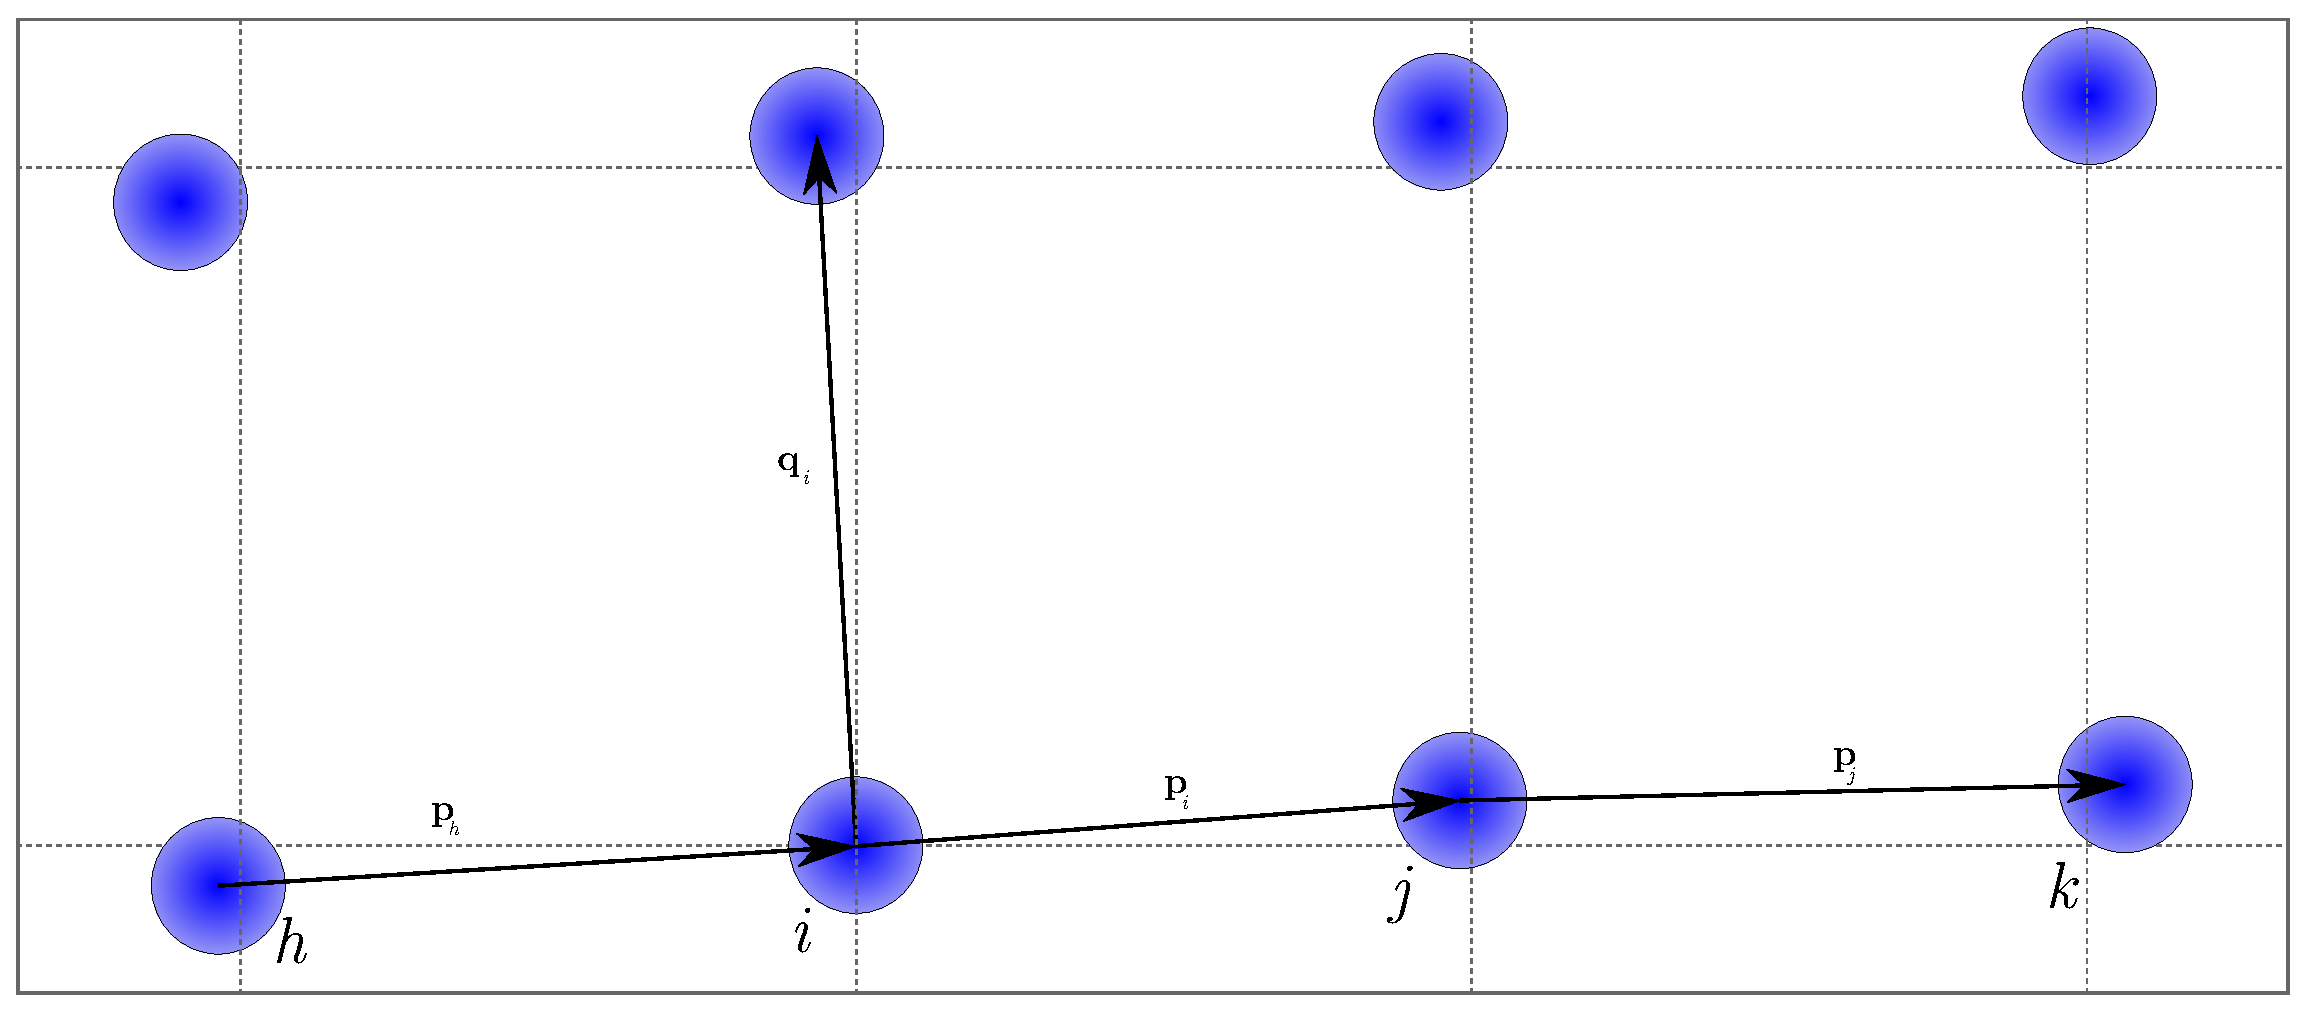
\includegraphics[width=\textwidth]{bonds}
\caption[Strained bonds in a dislocated crystal.]{The bonds that are considered for the $i$th atom in a region of crystal away from the slip plane; there is one bond to the nearest neighbour in the positive $x$~direction, $\mathbf{p}_i$, and one to the nearest neighbour in the positive $y$~direction, $\mathbf{q}_i$, to avoid double counting.\label{fig:bonds} }
\end{figure}





However there is a problem with this formulation. This assumes that every bond would, in equilibrium, be parallel to either the $x$ or the $y$ axis. This assumption is valid for the original Peierls model in which only displacements parallel to the $x$ direction were considered but the logarithmic term here represents a change in lattice orientation with position. A more nuanced approach requires some estimate of the local lattice orientation, if this is not done then the logarithmic term in \autoref{eqn:displacements} will mean that the strain in each bond will diverge, increasing with increasing distance from the dislocation core, whereas in reality the strains must be largest at the core.

There are clearly many possible ways of estimating the local lattice resistance, one possible method is to take the ideal orientation of the bond parallel to the slip plane for a particular bond to be paralell to the bonds on either side, i.e. as shown in \autoref{fig:bonds} the ideal orientation of $\mathbf{p}_i$ would be  parallel to $(\mathbf{p}_h + \mathbf{p}_j)$. The ideal orientation for $\mathbf{q}_i$ can be taken to be at \SI{90}{\degree} to this. So $\mathbf{\hat{i}}$ and $\mathbf{\hat{j}}$ in \autoref{eqn:estimate_strains} can be replaced with 
\begin{align}
\mathbf{\hat{i}}' &= \frac{(\mathbf{p}_h + \mathbf{p}_j)}{|\mathbf{p}_h + \mathbf{p}_j|} \nonumber \\
\mathbf{\hat{j}}' &= {\mathbf{\hat{i}}' \times \mathbf{\hat{k}}}
\end{align}
and the strain tensor can be calculated for each atom/unit cell, and hence the strain energy for each unit cell.



\FloatBarrier
\subsubsection{Misalignment energy}
\FloatBarrier
At the slip plane there is clearly going to be a break down of method highlighted above. For an atom immediately below the slip plane the identification of the nearest neighbour above the slip plane is perhaps not obvious. If the bond is taken to be simply  to the nearest atom above the slip plane ambiguities can arise 
It is possible that there will be two atoms equally close above the slip plane and such a simple criterion can lead to some atoms being bonded more than once and some atoms not being bonded. 

Instead a less arbitrary and more predictable method is to use the initial positions and assume that the $i$th atom can be bonded to two atoms in the layer above the slip plane. Since initially the horizontal spacing between atoms is $b$ for all atoms the two atoms must be within an interval $x_i^0 - b < x \leq x_i^0 + b$, as shown in \autoref{fig:slip_plane}. The energy for atom $i$ can be estimated from the average of the two bonds $\mathbf{q}_{i,\text{b}}$ and $\mathbf{q}_{i,\text{f}}$

\begin{figure}
\centering
\begin{subfigure}{\textwidth}
\centering
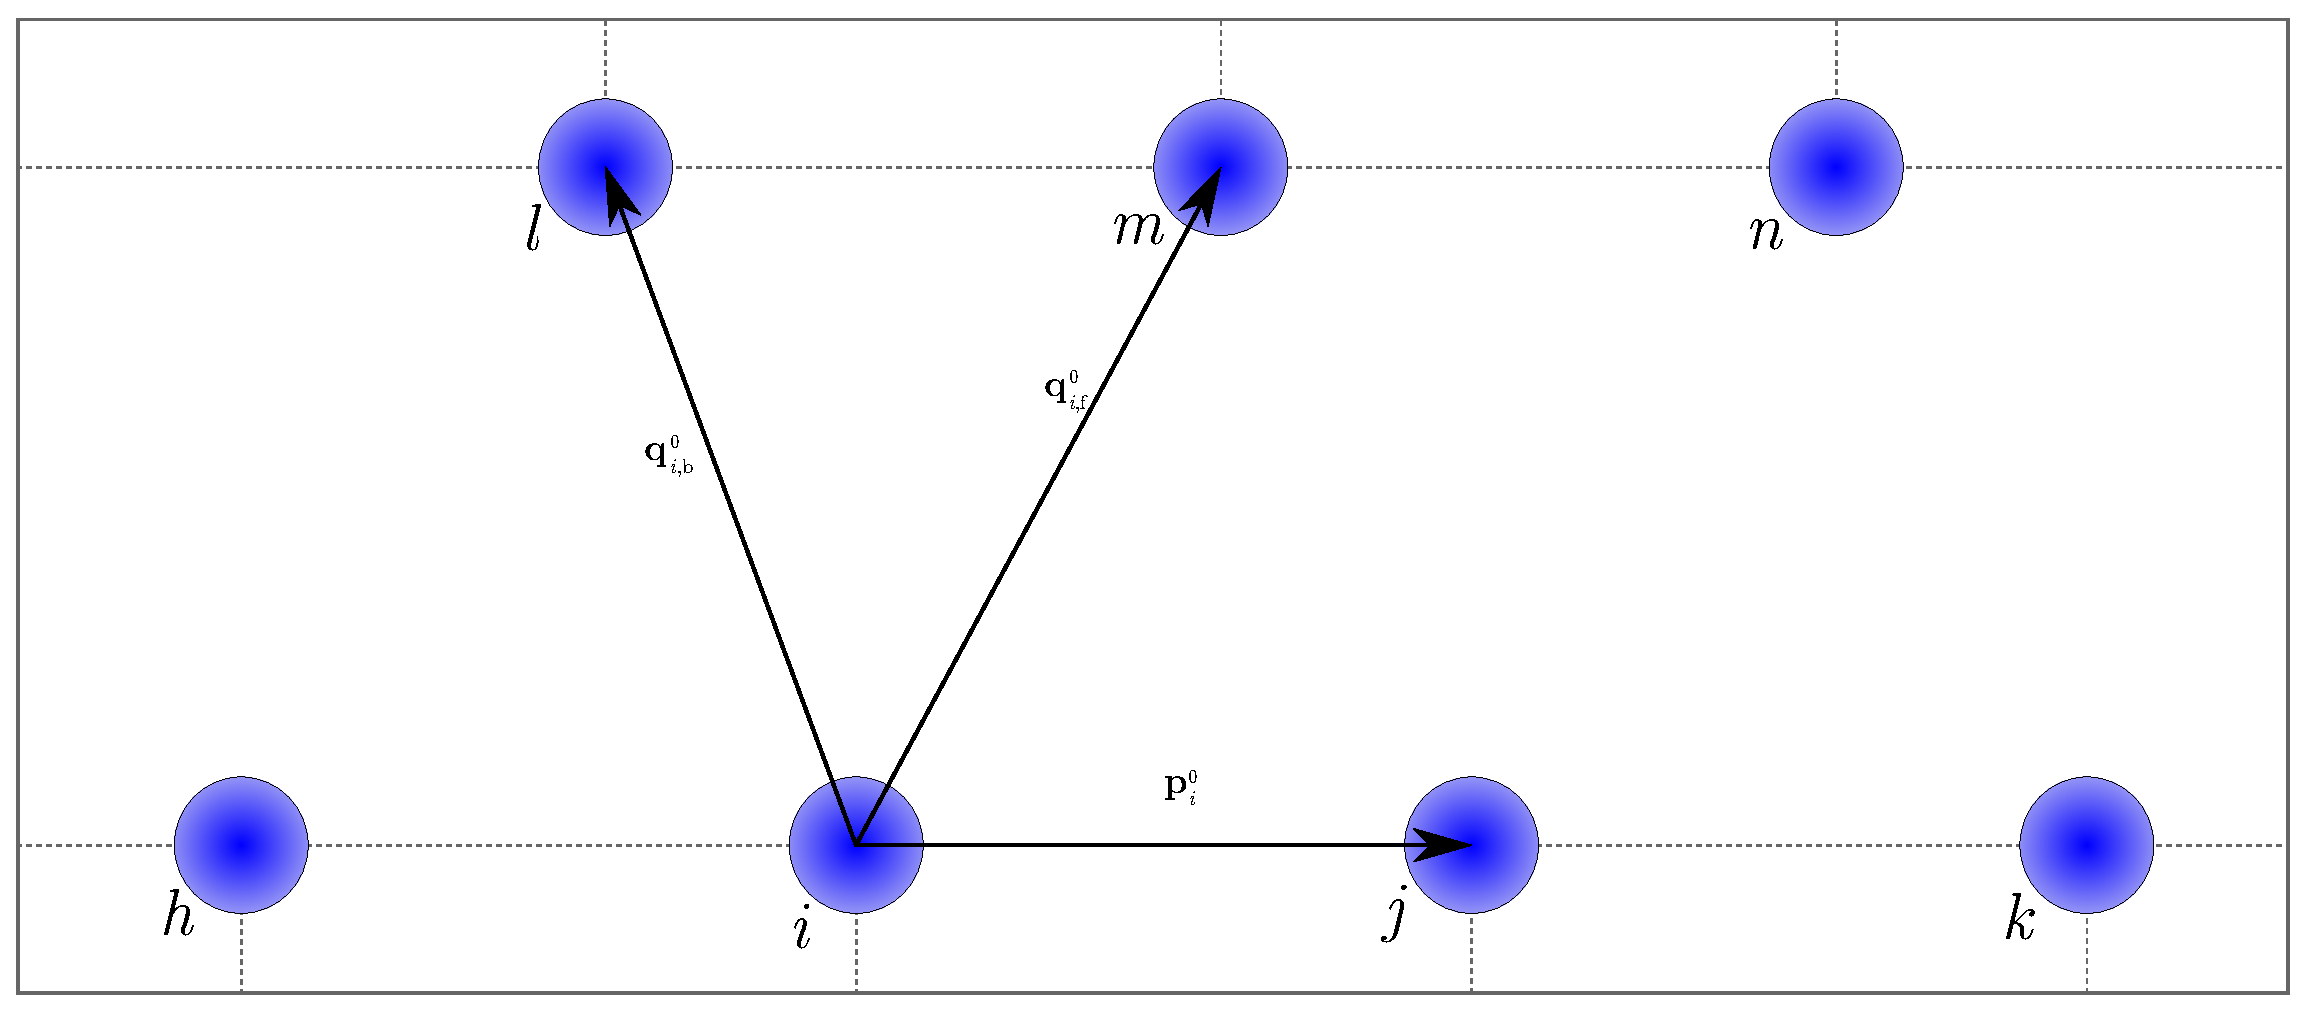
\includegraphics[width=\textwidth]{initial_slip_plane_bonds}
\caption{The initial positions of atoms either side of the slip plane.\label{fig:slip_plane_initial_positions}.}
\end{subfigure}
\par\medskip
\begin{subfigure}{\textwidth}
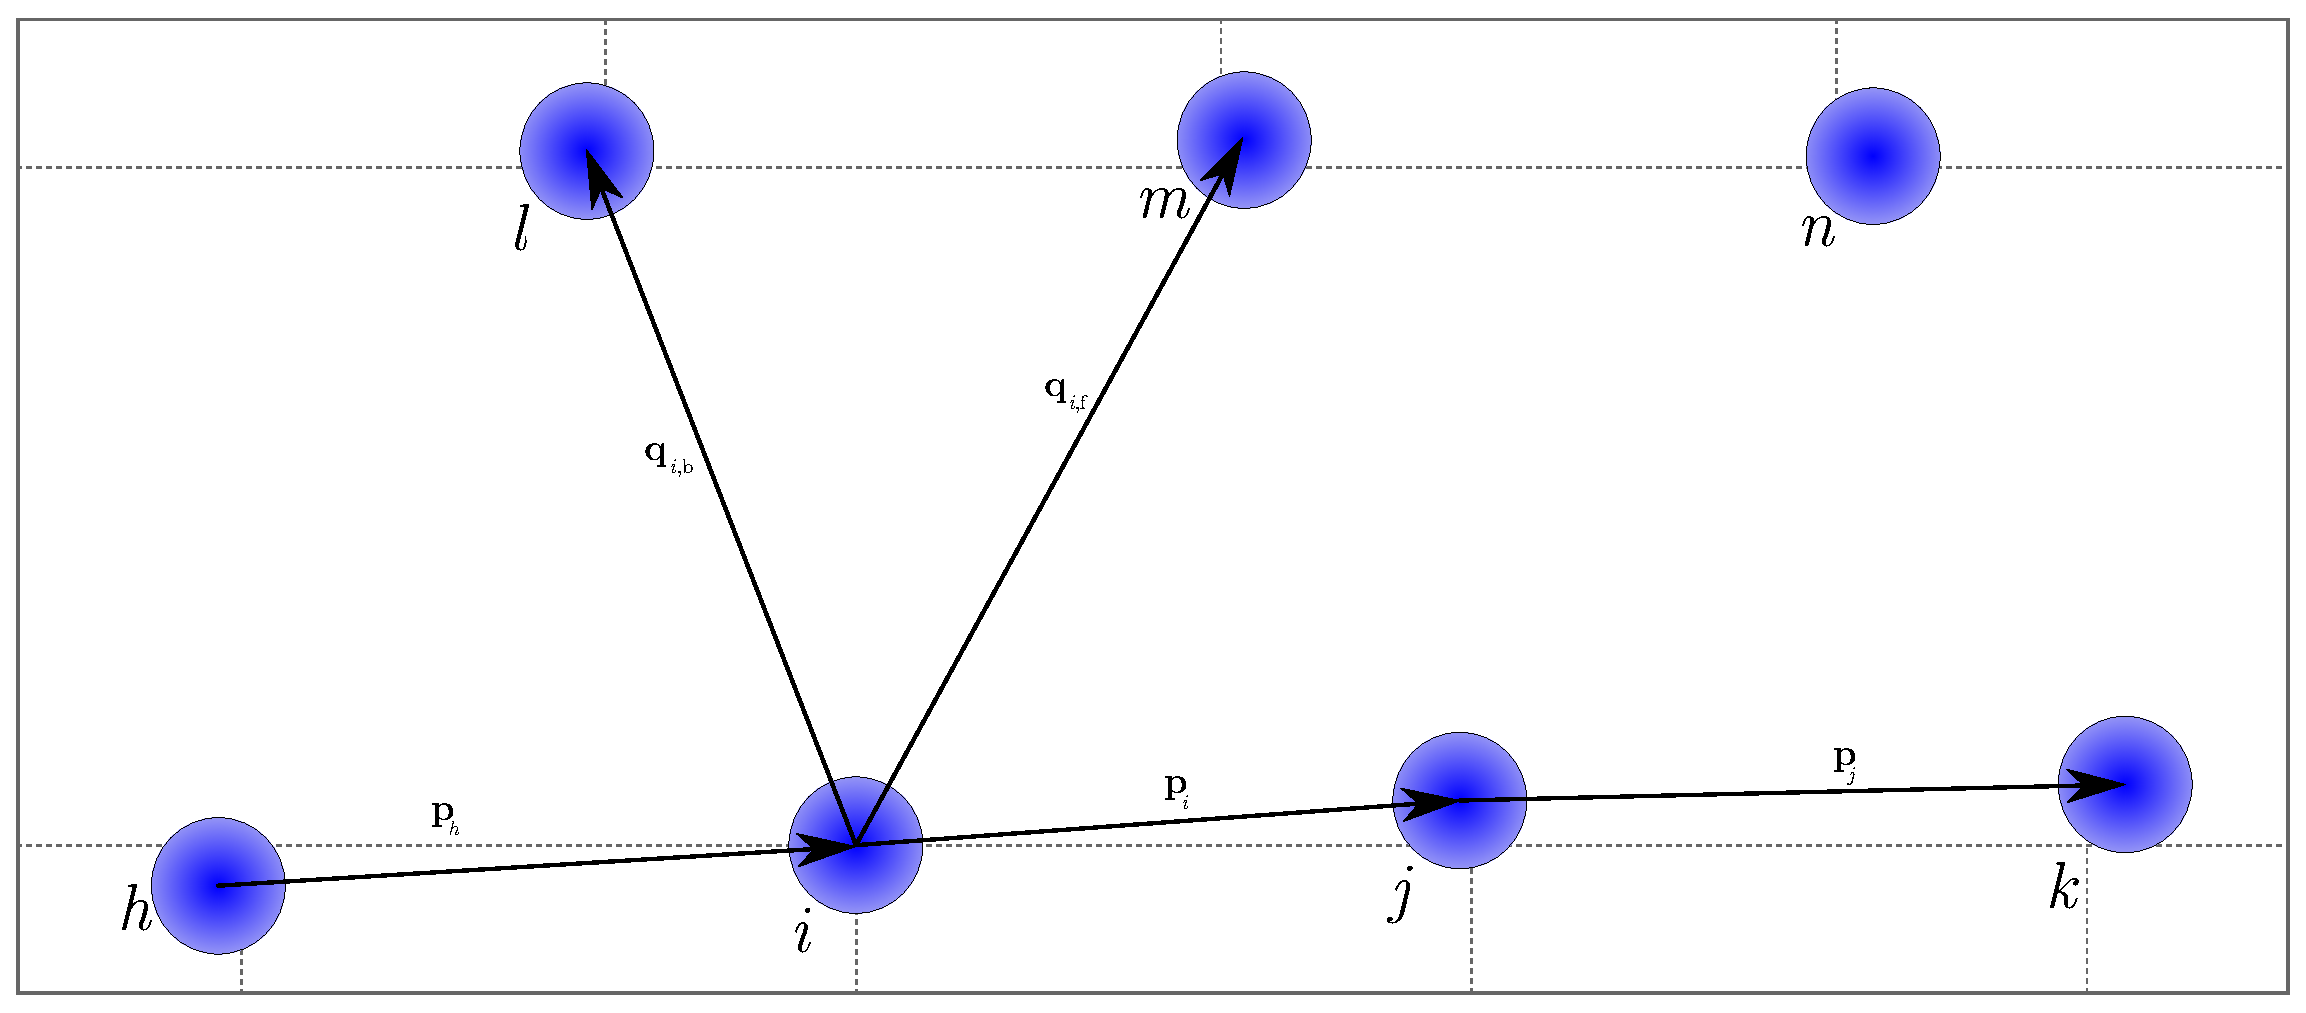
\includegraphics[width=\textwidth]{slip_plane_bonds}
\caption{The final positions of the atoms either side of the slip plane.\label{fig:slip_plane_final_positions}}
\end{subfigure}
\caption[Misaligned bonds cross the slip plane in a dislocated crystal.]{The slip plane before and after the application of the displacement field. The two atoms, $l$ and $m$, that can be considered bonded to the atom $i$ are shown along with the initial and final bonds, $\mathbf{q}_{i,\text{b}}$ and $\mathbf{q}_{i,\text{f}}$ which are backwards and forwards in the $x$ direction respectively. Also shown are the bonds $\mathbf{p}_h$ and $\mathbf{p}_j$ which are required to estimate the local orientation of the slip plane. \label{fig:slip_plane}}
\end{figure}


There are several methods to calculate the misaligned bonds. The simplest is to use the Frenkel approximation which, for an isotropic elastic material is 
\begin{equation}
U_i^\text{mis} = \frac{Gb^2}{4\pi^2} \left[\frac{d}{b}\right] \left[ 1 - \cos \left( \frac{2 \pi \phi}{d} \right) \right]
\end{equation}

which in terms of single crystal elastic constants takes $G=C_{66}$ (in Voigt notation see \cite{kelly_knowles2012chapter6_stress_strain}).

A more complete method for the calculation of the energy is to use the generalised stacking fault energy. Density functional theory can be used to calculate the energy of a stacking fault at an arbitrary misalignment. This is calculated by applying a displacement to two half crystals in a DFT simulation with periodic boundary conditions which introduces two opposing planar faults. The displacement is applied along the Burgers vector and the atoms are allowed to relax perpendicular to that displacement. Although the displacement field does not include any lateral (i.e. parallel to the lone vector) motion, allowing the DFT simulation of the stacking faults to relax laterally means that the energetic implications of lateral motion are included in the misalignment potential, although with an implicit assumption that the strains along the line vector do not extend beyond the slip plane. 

The energy changes with respect to a perfect crystal were considered and fitted with a simple empirical function:
\begin{equation}
\gamma(\phi) = \sum^{M}_{m=1} C_m \left[ 1 - \cos \left( \frac{2m\pi \phi}{b} \right) \right]
\end{equation}
where $\phi$ is the misalignment in the same units as the Burgers vector $b$, $m$ is an integer from \num{1} to $M$ and $C_m$ are coefficients fitted by a least-squares method to the energies calculated by DFT for different values of $\phi$. This is in units of \si{\joule\per\square\meter}, so a factor of $b$ must be applied to convert to a line energy in \si{\joule\per\meter}.


%%%%%%%%%%%%%%%%%%%%%%%%%%%%%%%%%%%%%%%%%%%%%%%%%%%%%%%%%%%%%%%5555%%%%%%%%%%%%%%%%%%%%%%%%%%%%%%%%%%%%%%%%%






%%%%%%%%%%%%%%%%%%%%%%%%%%%%%%%%%%%%%%%%%%%%%%%%%%%%%%%%%%%%%%%%%%%%%%%%%%%%%%%%%%%%%%%%%%%%%%%%%%%




\subsection{Empirical potentials}

Some materials can be described in a more physically insightful way than linear elasticity; as described in \autoref{sec:empirical_potentials}, empirical potentials have been developed for the field of molecular dynamics to be computationally convenient while at the same time approximating reality to a sufficient degree to gain insight into a system \cite{martinez2013}. One way to incorporate such potentials into the Peierls model described here is to write a simple python implementation of the potentials using the SciPy and NumPy packages and associated tools \cite{Numpy2011,Ipython2007,Millman2007,SciPy2001}; another way is to use the Atomic Simulation Environment \cite{ASE2017} or the python interface to the LAMMPS software package \cite{Plimpton1995,LAMMPS_web}.



To demonstrate the principle of using more physically informed potentials and hopefully capture more details of the energy changes as dislocations move the ionic solids were investigated using the Lennard-Jones potential:
\begin{equation}
\phi_{ij}(r_{ij}) = 4\epsilon_{ij} \left[ \left( \frac{\sigma_{ij}}{r_{ij}}\right)^{12}-     \left( \frac{\sigma_{ij}}{r_{ij}}\right)^6   \right]
\end{equation}
where $\epsilon_{ij}$ is the depth of the energy well and $\sigma_{ij}$ is the radius at which the energy is equal to zero or in the A--B form:
\begin{equation}
\phi_{ij}(r_{ij}) = \frac{A_{ij}}{r_{ij}^{12}} - \frac{B_{ij}}{r_{ij}^{6}}
\end{equation}
where $A_{ij} = 4\epsilon_{ij}\sigma_{ij}^{12}$ and $B_{ij} = 4 \epsilon_{ij} \sigma_{ij}^{6}$. The energy for any two atoms is then 
\begin{equation}
U_{ij}(r_{ij}) = \frac{1}{4\pi\epsilon_0} \frac{q_i q_j}{r_{ij}} + \frac{A_{ij}}{r_{ij}^{12}} - \frac{B_{ij}}{r_{ij}^{6}}
\end{equation}
where $\epsilon_0$ is the permittivity of free space.

The Lennard-Jones has been chosen as a simple example to demonstrate the application of empirical potentials for which fitted parameters are readily available \cite{Mao2014} and applicable to a class of materials for which the dislocation properties are not well explained by linear elasticity, the alkali halides.



\begin{table}
\centering
  \begin{tabular}{| m{3cm} | d{4} | d{-1} |}
  \hline
   Ion \rule{0pt}{3ex} & \multicolumn{1}{c|}{$\sigma_i$/\si{\angstrom}} & \multicolumn{1}{c|}{$\epsilon_i$/\si{\joule\per\mole}  }\\ \hline
   \ce{Li+} \rule{2ex}{0pt} & 1.715 & 241.25 \\
   \ce{Na+} & 2.497 & 327.44 \\
   \ce{K+} & 3.184 & 494.97 \\
   \ce{Rb+} & 3.302 & 1006.25 \\
   \ce{Cs+} & 3.440 & 2097.44 \\
   \ce{F-} & 3.954 & 27.05 \\
   \ce{Cl-} & 4.612 & 104.68 \\
   \ce{Br-} & 4.812 & 150.46  \\
   \ce{I-} & 5.197  & 176.56 \\
  \hline
  \end{tabular}
\caption[Lennard-Jones parameters.]{\rule[3ex]{0pt}{0pt} Parameters used for Lennard-Jones calculations from \cite{Mao2014}.\label{tab:LJ_params}}
\end{table}


The parameters used for the Lennard-Jones potential are shown in \autoref{tab:LJ_params}. They are calculated for each ion individually, to best reproduce lattice properties, and must be combined according to Lorentx-Berthelot rules:
\begin{align}
\epsilon_{ij} &= \sqrt[]{\epsilon_i \epsilon_j} \nonumber\\
\sigma_{ij} &= \frac{\sigma_i + \sigma_j}{2}
\end{align}

A na\"{\i}ve brute force implementation is given in Section~\ref{sec:ionic_energy_code} and an example input file is given for LAMMPS in Section~\ref{sec:lammps_input}. The LAMMPS pair style used was ``\texttt{lj/long/coul/long}'', the parameters for which are given in the example input file and is described in the LAMMPS documentation in \cite{LAMMPS_web}.

































































\section{Results and Discussion}

\subsection{Elastic Energy Calculations}
\label{sec:elastic_results}

The equilibrium dislocation configuration for a given dislocation position was calculated by optimisation of the dislocation structure with respect to the calculated energy, the sum of the strain energy in the half crystals either side of the slip plane and the misalignment energy in the slip plane. As discussed in \autoref{sec:optimisers} the choice of optimiser is affected by the behaviour of the function. The BFGS was found to be faster than the Nelder-Mead, though both algorithms produced very similar results, within the tolerance set for the algorithms to terminate. It was found that the tolerance of the optimisation algorithm had to be set very tight to achieve consistent results, a relative tolerance of around \num{1e-7}, because small changes in the energy are being studied. 

The variation of the dislocation energy with respect to the dislocation parameters, as defined in \autoref{eqn:displacement_field}, was investigated. These calculations were performed for a dislocation in copper at $\alpha=0$. The simulation cell used extended to \num{800} Burgers vectors from the dislocation core, which is approximately \SI{0.4}{\micro\meter} across the whole simulation.

First the dislocation structure was optimised to find the equilibrium configuration, then the  various parameters were varied away from these equilibrium values individually. The results are shown in \autoref{fig:variation_of_U_with_params}. 


\begin{figure}
\centering
\begin{subfigure}{0.4\textwidth}
\centering
\includegraphics[width=\textwidth]{U_vs_w}
\caption{The variation in the dislocation energy with the dislocation width.\label{fig:U_vs_w}}
\end{subfigure}
~
\begin{subfigure}{0.4\textwidth}
\centering
\includegraphics[width=\textwidth]{U_vs_c1}
\caption{The variation in the dislocation energy with the dislocation parameter $\mathbf{c_1}$.}
\end{subfigure}

\begin{subfigure}{0.4\textwidth}
\centering
\includegraphics[width=\textwidth]{U_vs_c2}
\caption{The variation in the dislocation energy with the dislocation parameter $\mathbf{c_2}$.}
\end{subfigure}
~
\begin{subfigure}{0.4\textwidth}
\centering
\includegraphics[width=\textwidth]{U_vs_c3}
\caption{The variation in the dislocation energy with the dislocation parameter $\mathbf{c_3}$.}
\end{subfigure}
\captionsetup{width=0.9	\textwidth,font={sf,scriptsize},labelfont=bf}
\caption[The variation of the calculated dislocation energy with the parameters of the displacement field.]{The variation of the calculated energy of a dislocation in copper at the $\mathbf{\alpha=0}$ position, calculated for a simulation extending \SI{0.4}{\micro\meter} from the dislocation core. The parameters are as defined in \autoref{eqn:displacement_field}. Only one parameter was varied at a time, all the others were held constant at their equilibrium values. The total energy is the solid black line, the strain energy in the two half crystals is the dashed red line and the misalignment energy in the slip plane is the dotted blue line. \label{fig:variation_of_U_with_params}}
\end{figure}


\begin{table}
\centering
\begin{tabular}{ l c c c }
\hline
\rule[2.5ex]{0pt}{0pt}Parameter                & Ideal             & Simulated $\alpha=0$  & Simulated $\alpha=0.5$  \\
\hline
$w$ (\si{\angstrom})  \rule[2.5ex]{0pt}{0pt}   & 1.581             & 2.441                 & 2.431 \\
$c_1$ (\si{\angstrom})                         & 0.308             & 0.36268                & 0.36270 \\
$c_2$ (\si{\angstrom})                         & 0.308             & 0.293070               & 0.293075 \\
$c_3$ (\si{\angstrom}) \rule[-0.5ex]{0pt}{0pt} & -0.0493           & -0.061864               & -0.061862 \\
Energy (\si{J/m})                              &  \num{1.56795e-9} & \num{1.20965e-08}      & \num{1.20963e-08} \\
\hline
\end{tabular}
\caption[A comparison between the ideal and simulated dislocation parameters]{A comparison of the ideal dislocation parameters and those found by optimising the energy of a simulated dislocation.\label{tab:dislocation_params}}
\end{table}

As expected all the parameters showed a single minimum and the variation was smooth, so a variational approach is applicable and the optimiser is likely to be reliable, i.e. the lowest energy configuration can be said to be the configuration a dislocation would take. 






The values of these parameters have simple solutions for the case of an isotropic elastic medium, these are given in \autoref{eqn:half_width} and \autoref{eqn:expressions_for_the_ideal_disloca_parameters}. These only depend on the Poisson's ratio, which for copper is \num{\sim0.34} \cite{Koster1961}, and the lattice parameters. These ideal values are compared with the optimised values in \autoref{tab:dislocation_params}. While the energy of the dislocation is higher than the expected value of $^1\!/_2\, G b^2$, approximately $4Gb^2$, the values of the dislocation configuration parameters are similar to the ideal values. In particular the atomistic model differs from the isotropic elastic continuum in that the values of the parameters vary as a function of $\alpha$ and the symmetry between $c_2$ and $c_3$ is broken.

The small variations in the values of the dislocation parameters and the dislocation energy, both as relative and absolute values,  as $\alpha$ varies require that a tight tolerance is used in their optimisation, and that care is taken in the computation not to introduce errors. If the tolerance is not tight enough then this would manifest as noise that depends on the initial guess to start the optimisation search, or the exact choices of parameters in the optimisation algorithm. This apparent noise would be deterministic but unpredictable so would to appear random.





\begin{figure}
\centering
% \begin{subfigure}{\textwidth}
% \centering
% \includegraphics[width=0.6\textwidth]{disloc_params_vs_alpha}
% \caption{The variation of the dislocation configuration parameters, $\mathbf{w}$, $\mathbf{c_1}$, $\mathbf{c_2}$ and $\mathbf{c_3}$, as a function of $\mathbf{\alpha}$.}
% \end{subfigure}

\begin{subfigure}{0.45\textwidth}
\centering
\includegraphics[width=\textwidth]{w_vs_alpha}
\caption{The variation of the dislocation width, $w$, as a function of $\alpha$.}
\end{subfigure}
~
\begin{subfigure}{0.45\textwidth}
\centering
\includegraphics[width=\textwidth]{c1_vs_alpha}
\caption{The variation of the dislocation width, $c_1$, as a function of $\alpha$.}
\end{subfigure}

\begin{subfigure}{0.45\textwidth}
\centering
\includegraphics[width=\textwidth]{c2_vs_alpha}
\caption{The variation of the dislocation width, $c_2$, as a function of $\alpha$.\label{fig:c2_vs_alpha}}
\end{subfigure}
~
\begin{subfigure}{0.45\textwidth}
\centering
\includegraphics[width=\textwidth]{c3_vs_alpha}
\caption{The variation of the dislocation width, $c_3$, as a function of $\alpha$.}
\end{subfigure}

\caption[The variation of the dislocation configuration parameters as a function of the dislocation position.]{The variation of the dislocation configuration parameters with $\mathbf{\alpha}$. Only small changes in the parameters were seen, the largest changes were seen in $w$ and the smallest in $\mathbf{c_3}$. The parameter all vary smoothly and approach $\mathbf{\alpha=0, 0.5}$ with no gradient, as required for equilibrium. Some noise was observed in the value of $\mathbf{c_2}$ and $\mathbf{c_3}$. \label{fig:disloc_params_vs_alpha}}
\end{figure}


The variation of the dislocation parameters and the dislocation energy were investigated by randomly sampling $\alpha$ in the range \numrange{0}{0.5} and optimising the dislocation configuration to give the lowest energy. The variation is the dislocation configuration parameters is given in \autoref{fig:disloc_params_vs_alpha}, while the variation of the total energy is given in \autoref{fig:Copper_U_tot_vs_alpha} and the relative changes in the different energy components is shown in \ref{fig:copper_800_rel_energies}.

An important observation is that the periodicity of the dislocation energy, and indeed the dislocation configuration, predicted by this model is $b$, not $^b\!/_2$ as predicted by \citet{Peierls1940,Clegg2006}. As discussed in \autoref{chap:plastic_deformation}, this is expected based on the symmetry inherent in the model. 

Peierls introduced an implicit symmetry by assuming that the dislocation configuration does not change as the dislocation moves and thus predicted a period of $^b\!/_2$. The formulation was changed by \citet{Huntington1955} to predicted a period of $b$. The model presented by \citet{Clegg2006} included an implicit symmetry since motion of atoms was limited to the slip direction and the strain energy was calculated from strains in the atomic bonds rather than as an integral over an elastic medium. This meant that there was no distinction between the atoms above the slip plane and the atoms below the slip plane, and thus no distinction between the $\alpha = 0$ and $\alpha = 0.5$ position. The current model has no such symmetry across the slip plane, due to the logarithmic term in \autoref{eqn:displacement_field}, and so the periodicity of $b$ is expected.

The dislocation parameters vary smoothly from $\alpha = 0$ to $\alpha = 0.5$ and approach the two equilibrium positions with zero gradient as required by equilibrium. There is some noise in the value of $c_2$, as shown in \ref{fig:c2_vs_alpha}. This is likely due to the changes in the dislocation parameters being close to the tolerance of the optimisation algorithm. This is not sufficiently noisy to present a problem, but highlights the need for care in deciding the trade off between computational time and the accuracy of the calculated values.



\begin{figure}
\captionsetup{width=0.6\textwidth,font={sf,scriptsize},labelfont=bf}
\centering
\includegraphics[width=0.5\textwidth]{Copper_800_U_tot}
\caption[Energy variation of a dislocation in copper with the dislocation position.]{The variation of the dislocation energy with position for a dislocation in copper. The results shown are for a model including atoms to a distance of 800 Burgers vectors from the dislocation core, i.e. a distance of $\sim$\SI{300}{\nano\metre}.  Note that the changes in energy are small relative to the absolute value of the dislocation energy.\label{fig:Copper_U_tot_vs_alpha}}
\end{figure}

The variation of the energy with $\alpha$, \autoref{fig:Copper_U_tot_vs_alpha}, was qualitatively as expected from previous work \cite{Bulatov1997,Clegg2006}, a smooth but very small variation in the energy, some five orders magnitude smaller than the value of the dislocation energy. The variation of the two components of the energy was also as expected. This is most easily seen as changes by setting the energy at $\alpha=0$ to be zero, as shown in \autoref{fig:copper_800_rel_energies}. The strain energy and the misalignment energy vary out of phase with the other, thus the two components of the energy experience larger variations than the total. It is also possible that the relative magnitude of the two components will alter which of the two equilibrium positions is stable an which is unstable.


\begin{figure}
\captionsetup{width=0.6\textwidth,font={sf,scriptsize},labelfont=bf}
\centering
\includegraphics[width=0.5\textwidth]{Copper_800_rel_energies}
\caption[The energy changes with dislocation position for  copper.]{The energy changes with position for a dislocation in copper showing the two components of the energy, the strain energy and the misalignment energy, and the total energy. This simulation extended \num{800} Burgers vectors from the dislocation core, or around \SI{04}{\micro\meter}.\label{fig:copper_800_rel_energies}}
\end{figure}




To undertake further analysis the energy variation can be fitted with a simple empirical function:
\begin{equation}
U = \sum^N_n C_n \cos (2 \pi n \alpha) \label{eqn:empirical_function}
\end{equation}
where $C_n$ are the parameters to be fitted, $n$ is an integer between $0$ and $N$ and $\alpha$ is the displacement of the dislocation from the initial position as a fraction of the Burgers vector. Usually it was found that $N=4$ gave a good fit to the calculated energy variations. Since this is an easily differentiable function the stress can be calculated in a straight forward manner from the gradient:
\begin{equation}
\tau = \frac{dU}{d\alpha} \frac{1}{lb^2}
\end{equation}
where $l$ is the length of dislocation line and $b$ is the Burgers vector. The gradient is readily calculated by
\begin{equation}
\frac{dU}{d\alpha} = \sum_n^N - 2 \pi C_n \sin ( 2 \pi n \alpha )
\end{equation}

The Peierls stress is the maximum value of the stress, which occurs at the point of maximum gradient $dU/d\alpha$. I.e. where
\begin{equation}
\frac{d^2U}{d\alpha^2} = \sum_n^N -4 \pi^2 n^2 C_n \cos ( 2 \pi n \alpha ) = 0
\end{equation}

A script was written to do this fitting and gradient calculation automatically, the code is included in \autoref{sec:analysing_results_code}. An example of this sort of fit is shown in \autoref{fig:empirical_fit}. For the example of copper above this yields a Peierls stress of \SI{8.98}{\mega\pascal} or as a fraction of the shear modulus, \num{2.54e-4}\,$G$. This is approximately 10 times larger than the value estimated by experiment \cite{Wang1996}.

\begin{figure}
\centering
\includegraphics[width=0.5\textwidth]{Empirical_Fit}
\captionsetup{width=0.6\textwidth,font={sf,scriptsize},labelfont=bf}
\caption[Empirical fit to the variation in energy with dislocation position.]{Empirical fit to the variation in energy with dislocation position using 4 terms. The fit is good, so can be reliably used for further analysis.\label{fig:empirical_fit}}
\end{figure}


To characterise the dependence of the model on the volume of crystal modelled, various simulation sizes were modelled for dislocations in copper. The size here is the range about the core of the dislocation in the slip direction and normal to the slip planes, while symmetry was exploited along the dislocation line to model only one repeat unit. The resulting simulated crystal therefore has a rectangular cross-section, rather than, say, cylindrical.

%Schematic?

\begin{figure}
\centering
\begin{subfigure}{0.4\textwidth}
\centering
\includegraphics[width=\textwidth]{Tp_vs_size}
\caption{The variation of the calculated Peierls stress with simulation size.}
\end{subfigure}
~
\begin{subfigure}{0.4\textwidth}
\centering
\includegraphics[width=\textwidth]{Energy_vs_size}
\caption{The variation of the calculated dislocation line energy with the simulation size and a best fit line for a logarithmic function.\label{fig:energy_vs_size}}
\end{subfigure}
\captionsetup{width=0.9\textwidth,font={sf,scriptsize},labelfont=bf}
\caption[The variation of the calculated Peierls stress and dislocation line energy with simulation size.]{Plots characterising the sensitivity of the model to the simulation size. The value of the Peierls stress is quite quickly converged to a constant, the energy in fact increases logarithmically, as shown by the best fit line.\label{fig:effect_of_size_on_simulation}}
\end{figure}

\begin{figure}
\captionsetup{width=0.6\textwidth,font={sf,scriptsize},labelfont=bf}
\centering
\includegraphics[width=0.5\textwidth]{tp_vs_d_b}
\caption[A comparison of predicted Peierls Stresses against experimental estimates and a previous model.]{A comparison of predicted Peierls Stresses against experimental estimates \cite{Wang1996} and a previous model \cite{Clegg2006} for an isotropic material, the highest for a screw dislocation and the others are for edge dislocations where $\nu=$ 0.1, 0.2 and 0.3. \label{fig:tp_vs_d_b}}
\end{figure}


The energy and Peierls stresses were calculated and are presented in \autoref{fig:effect_of_size_on_simulation}. The effects of size are limited to a small range for this elastic simulation, with the Peierls stress converging to \SI{1}{\percent} when the simulation is  \SI{\sim 30}{\nano\meter} across, which is around a hundred Burgers vectors.

The variation of energy with respect to simulation size does not converge, as can be seen in \autoref{fig:energy_vs_size}. However this is expected; as derived by \citet{Nabarro1947} the energy of a single dislocation in an otherwise perfect cylindrical crystal will vary logarithmically with the radius of the crystal. A best fit line is shown in \autoref{fig:energy_vs_size}, with an equation of the form
\begin{equation}
y = c_1 + c_2 \log \left( x \right)
\end{equation}
which fits the results well. This is seen in the current work because the displacement field, \ref{eqn:displacement_field},  includes a logarithmic term, whereas previous models have usually been limited to displacements parallel to the slip direction, at least in the far field.



The Peierls stress was calculated for a number of phases  and compared with experiment and previous models and are shown in \autoref{fig:tp_vs_d_b}. As can be seen the qualitative trends are preserved, with the same trend in Peierls stress with lattice geometry observed. However the values predicted systematically differ from experiment, at low values of $d/b$ the current model underestimates the Peierls stress and at high values of $d/b$ the model overestimates the Peierls stress. This limits the use of the model as a quantitative predictive tool, but should allow qualitative comparisons to be undertaken.

The effect of changes in the single crystal elastic tensor were assessed for the \ce{Fe3C} structure, cementite. Work by Miles Stopher and David Bombac on the effects of hydrogen embrittlement in steels have assessed the effects of hydrogen on the elastic tensor \cite{Stopher2017}. It is expected from experiment \cite{Stopher2017} that a softening of the cementite phase occurs, allowing dislocation mediated dissolution. The elastic tensors for the four compositions, \SI{0}{at\percent}, \SI{5}{at\percent}, \SI{7}{at\percent}, \SI{10}{at\percent} hydrogen, that were investigated are given in \autoref{sec:elastic_tensors}.



The Peierls analysis results are shown in \autoref{fig:tp_cementite}. There is little to no change in the Peierls stress at hydrogen loadings of below \SI{7}{\percent}, is a clear and large drop in the Peierls stress for cementite between \SI{7}{\percent} and \SI{10}{\percent}. While, as seen earlier, the quantitative results of the model may not be directly comparable with experiment, the relative changes in behaviour are reliable. This is supportive of the idea that cementite is softened by the addition of hydrogen.
\begin{figure}
\captionsetup{width=0.6\textwidth}
\centering
\includegraphics[width=0.5\textwidth]{Peierls_Stress_Cementite}
\caption{The effect of hydrogen loading on the predicted Peierls stress of cementite on the [100](010) slip system.\label{fig:tp_cementite}}
\end{figure}


\FloatBarrier
\subsection{Dislocations in ionic solids}
\FloatBarrier


Energy changes in ionic solids were fitted with an empirical function in a similar manner to that described in \autoref{sec:elastic_results} except now the energy components are not misalignment and strain energy terms but electrostatic and short-range terms. This was done for the two slip systems known to operate in crystals with the rocksalt structure, the <110>\{001\} and the <110>\{1\={1}0\}.


First the energy was calculated via a python program, included in \autoref{sec:ionic_energy_code}, that used a very simple approach, calculating the energy for all the interactions in the crystal with no cut offs. This gives the energy without the risk of artefacts that can be introduced by cut offs, but at the cost of computational time.


The energy changes calculated in this way, using the same optimisation procedure as described above, are shown in \ref{fig:NaCl_energy_changes}. There is a curious result that the periodicity appears to be different for the two dislocations, a period of $b$ for the <110>\{1\={1}0\} slip system and $^b\!/_2$ for the <110>\{001\} slip system. This can be explained in terms of the crystal structure and symmetry inherent to the two slip systems. Considering the core structures shown in \autoref{fig:Schematic_NaCl_dislocs}, for the <110>\{001\} slip system the $\alpha=0.5$ position is equivalent to the $\alpha=0$ position because the structure will be mirrored through the plane normal to the slip direction and passing through the dislocation core. This contrasts with the symmetry in the original Peierls model which was based on the structure being mirrored through the slip plane. The same symmetry does not exist for the <110>\{1\={1}0\} slip system, so the period is $b$.

\begin{figure}
\centering
\begin{subfigure}{0.4\textwidth}
\centering
\includegraphics[width=\textwidth]{NaCl_110_001_U_vs_alpha}
\caption{The energy changes with displacement of a <110>\{001\} dislocation in NaCl.\label{fig:NaCl_110_001_energy_changes}}
\end{subfigure}
~
\begin{subfigure}{0.4\textwidth}
\centering
\includegraphics[width=\textwidth]{NaCl_110_110_U_vs_alpha}
\caption{The energy changes with displacement of a <110>\{1\={1}0\} dislocation in NaCl.\label{fig:NaCl_110_110_energy_changes}}
\end{subfigure}
\caption{The energy changes with position of dislocation in NaCl. Note that the scale of the energy changes is much larger for the <110>\{1\={1}0\} slip system.\label{fig:NaCl_energy_changes}}

\end{figure}



The data was fitted using the function given in \autoref{eqn:empirical_function}, and this gave the Peierls stress of the two systems as \SI{76.6}{\mega\pascal} for the <110>\{001\} slip system, and \SI{63.7}{\giga\pascal} for the <110>\{1\={1}0\} system. The value for <110>\{001\} system is in reasonable agreement with experimental measurements of the Peierls stress, \citet{Haasen1985} estimated the Peierls stress of this slip system to be \SI{140}{\mega\pascal}. The value for the <110>\{1\={1}0\} slip system is clearly not in agreement with the estimated Peierls stress of \SI{10}{\mega\pascal}.



The variation of the dislocation width is shown in \autoref{fig:NaCl_w_vs_alpha}. The period of the variation of the width for the two slip systems is the same as that of the energy variation. The <110>\{001\} slip system shpows the expected behaviour, small and smooth variation, \autoref{fig:NaCl_110_001_w_variation}, though there is some noise in the graph showing that perhaps the model has not fully converged on the lowest energy value. There is a much larger variation in the width for the <110>\{1\={1}0\} slip system, \ref{fig:NaCl_110_110_w_variation}, and there is a discontinuity in the value at around $\alpha=0.1$. This corresponds to the very steep part of the energy variation shown in \autoref{fig:NaCl_110_110_energy_changes}.


\begin{figure}
\centering
\begin{subfigure}{0.4\textwidth}
\centering
\includegraphics[width=\textwidth]{NaCl_110_001_w_vs_a}
\caption{The variation of the dislocation width with dislocation position for the <110>\{001\} slip system. \label{fig:NaCl_110_001_w_variation}}
\end{subfigure}
~
\begin{subfigure}{0.4\textwidth}
\centering
\includegraphics[width=\textwidth]{NaCl_110_110_w_vs_a}
\caption{The variation of the dislocation width with dislocation position for <110>\{1\={1}0\} slip system.\label{fig:NaCl_110_110_w_variation}}
\end{subfigure}
\caption[The variation of the dislocation width with position for the two slip systems of NaCl.]{The variation of the dislocation width with position for the two slip systems of NaCl. The <110>\{001\} slip system shows the expected behaviour, showing relatively small variation in a smooth and continuous manner. The <110>\{1\={1}0\} slip system shows a much larger variation and a rapid if not discontinuous change at around $\alpha=0.1$.\label{fig:NaCl_w_vs_alpha}}
\end{figure}

One problem with modelling dislocations in ionic materials is the computational complexity compared to the elastic case. There are a number of reasons that the computation takes much longer, the model must be three dimensional since the interactions are three dimensional. This means the number of atoms is larger. But also the calculation scales more quickly with the size of the simulation, since now there are $n^2$ energy calculations to do for $n$ atoms rather than simply $n$ for the elastic energy calculation. Thus despite using the excellent numerical python project \citep{Numpy2011} which is well optimised to efficiently undertake calculations the scale of the simulation was much more limited, extending only tens of nanometers rather than hundreds from the dislocation core. Given the inherently long range nature of the electrostatic interaction this is potentially insufficient.

To address this the model was adapted to use the LAMMPS \cite{LAMMPS_web} software package to undertake the energy calculation, using the coulombic and Lennard-Jones calculators built in to the LAMMPS package. An example script and input files are included in \autoref{sec:lammps_input}. The principle is much the same, though now the energy calculation is using the highly optimised LAMMPS routines, which relies on choosing appropriate parameters and settings, which was done according to the LAMMPS manual \cite{LAMMPS_web}. One particular advantage is the ability to employ periodic boundary conditions along the length of the dislocation line, thus removing potential artefacts that might arise from the termination of the dislocation.

The results for the <110>\{1\={1}0\} slip system are shown in \autoref{fig:NaCl_110_110_U_vs_a_LAMMPS}. The variation is quite similar to that found using the na\"ive python based energy calculator despite the periodic boundary conditions along the dislocation line and extending the simulation out from the core to \SI{\sim 100}{\nano\meter}. The maximum gradient of the best fit achievable using \autoref{eqn:empirical_function} gives the Peierls stress as \SI{63.8}{\giga\pascal}, which is very close to the the result from \autoref{fig:NaCl_110_110_energy_changes}. 


\begin{figure}
\centering
\includegraphics[width=0.5\textwidth]{NaCl_110_110_U_vs_alpha_LAMMPS}
\caption{The energy variation of a <110>\{1\={1}0\} dislocation in NaCl using the energy calculations available in LAMMPS. There is a lot of scatter, which does not appear to be random, but is likely due to insufficiently tight convergence criteria.\label{fig:NaCl_110_110_U_vs_a_LAMMPS}}
\end{figure}

The variation of the dislocation width with $\alpha$ is shown in \autoref{fig:LAMMPS_w_vs_a_NaCl}. There are some differences between the python based model adn the LAMMPS based model. Both models show a discontinuity in the width, dropping rapidly around $\alpha=0.1$, but the LAMMPS based model predicts zero width for $\alpha$ \numrange{\sim 0.1}{ 0.9}, where the python based model predicted an increase to a maximum at $\alpha=0.5$. This might be attributable to the size of the simulation or the termination of the dislocation since those are the principle differences between the two models.

\begin{figure}
\centering
\includegraphics[width=0.5\textwidth]{NaCl_110_110_w_vs_a_LAMMPS}
\caption{The variation of the dislocation width with position for the <110>\{1\={1}0\} slip system in NaCl.\label{fig:LAMMPS_w_vs_a_NaCl}}
\end{figure}




It therefore seems unlikely that simulation size or the termination of the dislocation at the free surface were major problems, instead some other factor is at fault. It is possible that core reconstruction occurs in NaCl such that the displacement field, \autoref{eqn:displacement_field}, is no longer appropriate. Other energetic considerations which have been neglected could be important, in particular the polarisability of atoms has not been modelled. There are net dipoles around the <110>\{1\={1}0\} dislocation in NaCl but not around <110>\{001\} dislocations, which could explain the discrepancy. Since the Peierls model only deals in relatively small changes of a large number small factors such as this can be important.


\section{Conclusions}

A parametrised form of the displacement field around an edge dislocation has been reached by adapting the solution for an isotropic elastic medium. This allows the construction of atomic configurations in three dimensions rather than one. This formulation also reduces the parameter space that must be searched for the optimal dislocation structure to a tractable size.

A series of python modules have been written to allow the modelling of dislocations in a variety of materials using a variational approach to minimise the energy of the atomic configuration for every dislocation position. The Peierls stress is calculated from the maximum gradient of the dislocation energy. The modular nature allows functionality to be added or altered easily. 

The first module builds the dislocation by constructing an array representation of atomic coordinates around the dislocation core via the adapted displacement field. This is deliberately left extensible to allow, for example, the addition of a screw dislocation or core reconstruction.

Two further modules have been written to calculate the energy of a dislocation as represented by an array of atomic coordinates. One builds on the existing Peierls models that use linear elasticity for strain energies away from the slip plane and a misalignment potential for the slip plane, either approximated as a sinusoid that obeys Hooke's law at low strains, or fitted empirically to \emph{ab initio} calulations of the $\gamma$-surface. This module extends the Peierls analysis to use the full stiffness tensor rather than simple elastic constants. The other uses the electrostatic interaction and the Lennard-Jones potential to calculate the energy of a dislocation in an ionic solid.

The elastic Peierls model is in agreement with the trends in material behaviour observed in experiment and predicted by previous models. However the effect of lattice geometry is not as strong in this model as in experiment, thus only qualitative conclusions can be drawn. The model does predict a softening of the cementite structure when hydrogen is added, as predicted by experiment.

The ionic Peierls model successfully predicts the behaviour of the <110>\{001\} slip system in \ce{NaCl} as observed by experiment. The electrostatic and short-range repulsion energy components vary out of phase with each other, in a parallel to the strain energy and misalignment energy in traditional Peierls models. The behaviour of the <110>\{1\={1}0\} slip system is not successfully predicted. It was shown that this was not due to the size of the simulation or the termination of the dislocation line at a free surface by the use of LAMMPS as an energy calculator, allowing much larger simulations and the use of periodic boundary conditions. Other explanations are the lack of polarisability in the atom potentials used or the possibility of dislocation core reconstruction, which was not treated by the model.





















